\section{Interactive Visual Analysis of Fiber Bundles}
In order to interactively analyze and explore the individual fiber bundles, we have applied the FiberScout visualization concept introduced by Weissenb{\"o}ck et al.~\cite{Weissenbock2014} to the MetaTracts. Figure~\ref{fig:metatracts_fiberscout_workflow} shows the necessary steps to realize the interactive fiber bundles analysis tool.

\begin{figure}[htb]
	\centering
	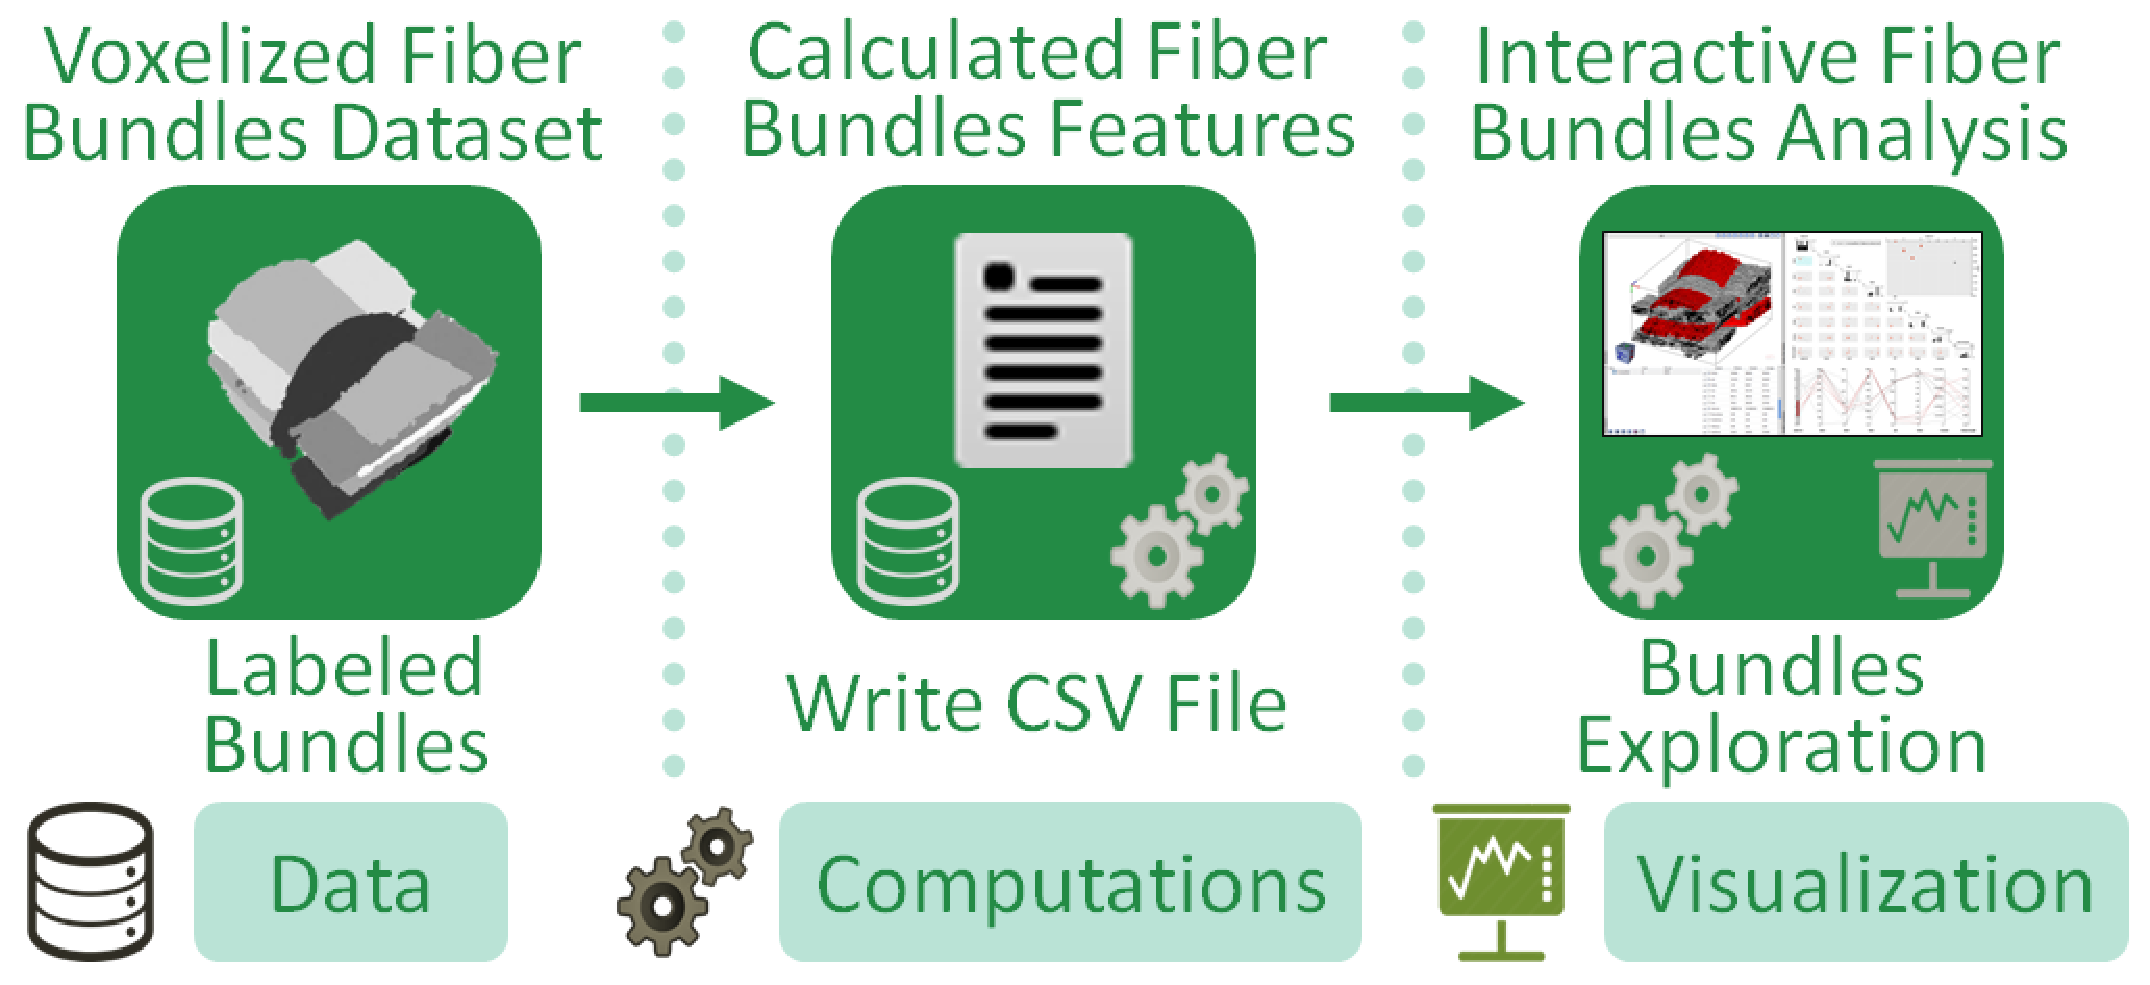
\includegraphics[width=\linewidth]{images/MetaTractsToFiberScout_workflow.eps}
	\caption{Flow chart of the interactive fiber bundles analysis tool.}
	\label{fig:metatracts_fiberscout_workflow}
\end{figure}

During the voxelization process (Sec.~\ref{subsec:voxel_surf_extraction}) a unique identification is assigned to each fiber bundle. Based on these labeled voxel data, we use ITK\cite{Ibanez2005} filters to calculate multiple interesting fiber bundles characteristics. With this additional information, the individual bundles are described in much more detail. According to the work of~\cite{Weissenbock2014} we used the following characteristics to describe the fiber bundles: the main diagonal elements of the orientation tensors ($a_{11}$, $a_{22}$, $a_{33}$), spherical coordinates of the orientations ($\varphi$, $\theta$), Cartesian coordinates of the centers ($X_{i}$, $Y_{i}$, $Z_{i}$) and the $volume$. Furthermore, we calculate the x, y, z bounding box dimensions and the major axis length of a fiber bundle. By combining the image data and the fiber bundles characteristics we were able to create an interactive tool which allows to select, classify and color-code the individual bundles based on the calculated characteristics.

The graphical user interface of the interactive tool is shown in Figure~\ref{fig:interactive_tool_gui}. A linked scatter plot matrix (D) and parallel coordinates (C) are used to assess the relationships between the different fiber bundles features. From the selected bundles classes can be created. The defined classes are managed in a list (B). In addition, statistical informations (min, mean, max) on the characteristics of a class are given. When performing a selection in the scatter plot matrix or the parallel coordinates as well as browsing through the classes or the sub elements of a class in the list the fiber bundles are immediately visualized in the 3D renderer (A).

Figure~\ref{fig:interactive_tool_gui} shows two fiber bundles classes (blue and orange) which are stored in the class list (A). The classifications ares based on the characteristic \textit{theta} (orientation to the Z-axis in \textdegree). The fiber bundles in the blue class are orientated around 90\textdegree to the Z axis, the fiber bundles in the orange class are oriented around 0\textdegree. The red selection presented in the scatter plot matrix (D), parallel coordinates (C) and the 3D renderer (A) defines two fiber bundles of the blue class, whereas....    

\begin{figure}[htb]
	\centering
	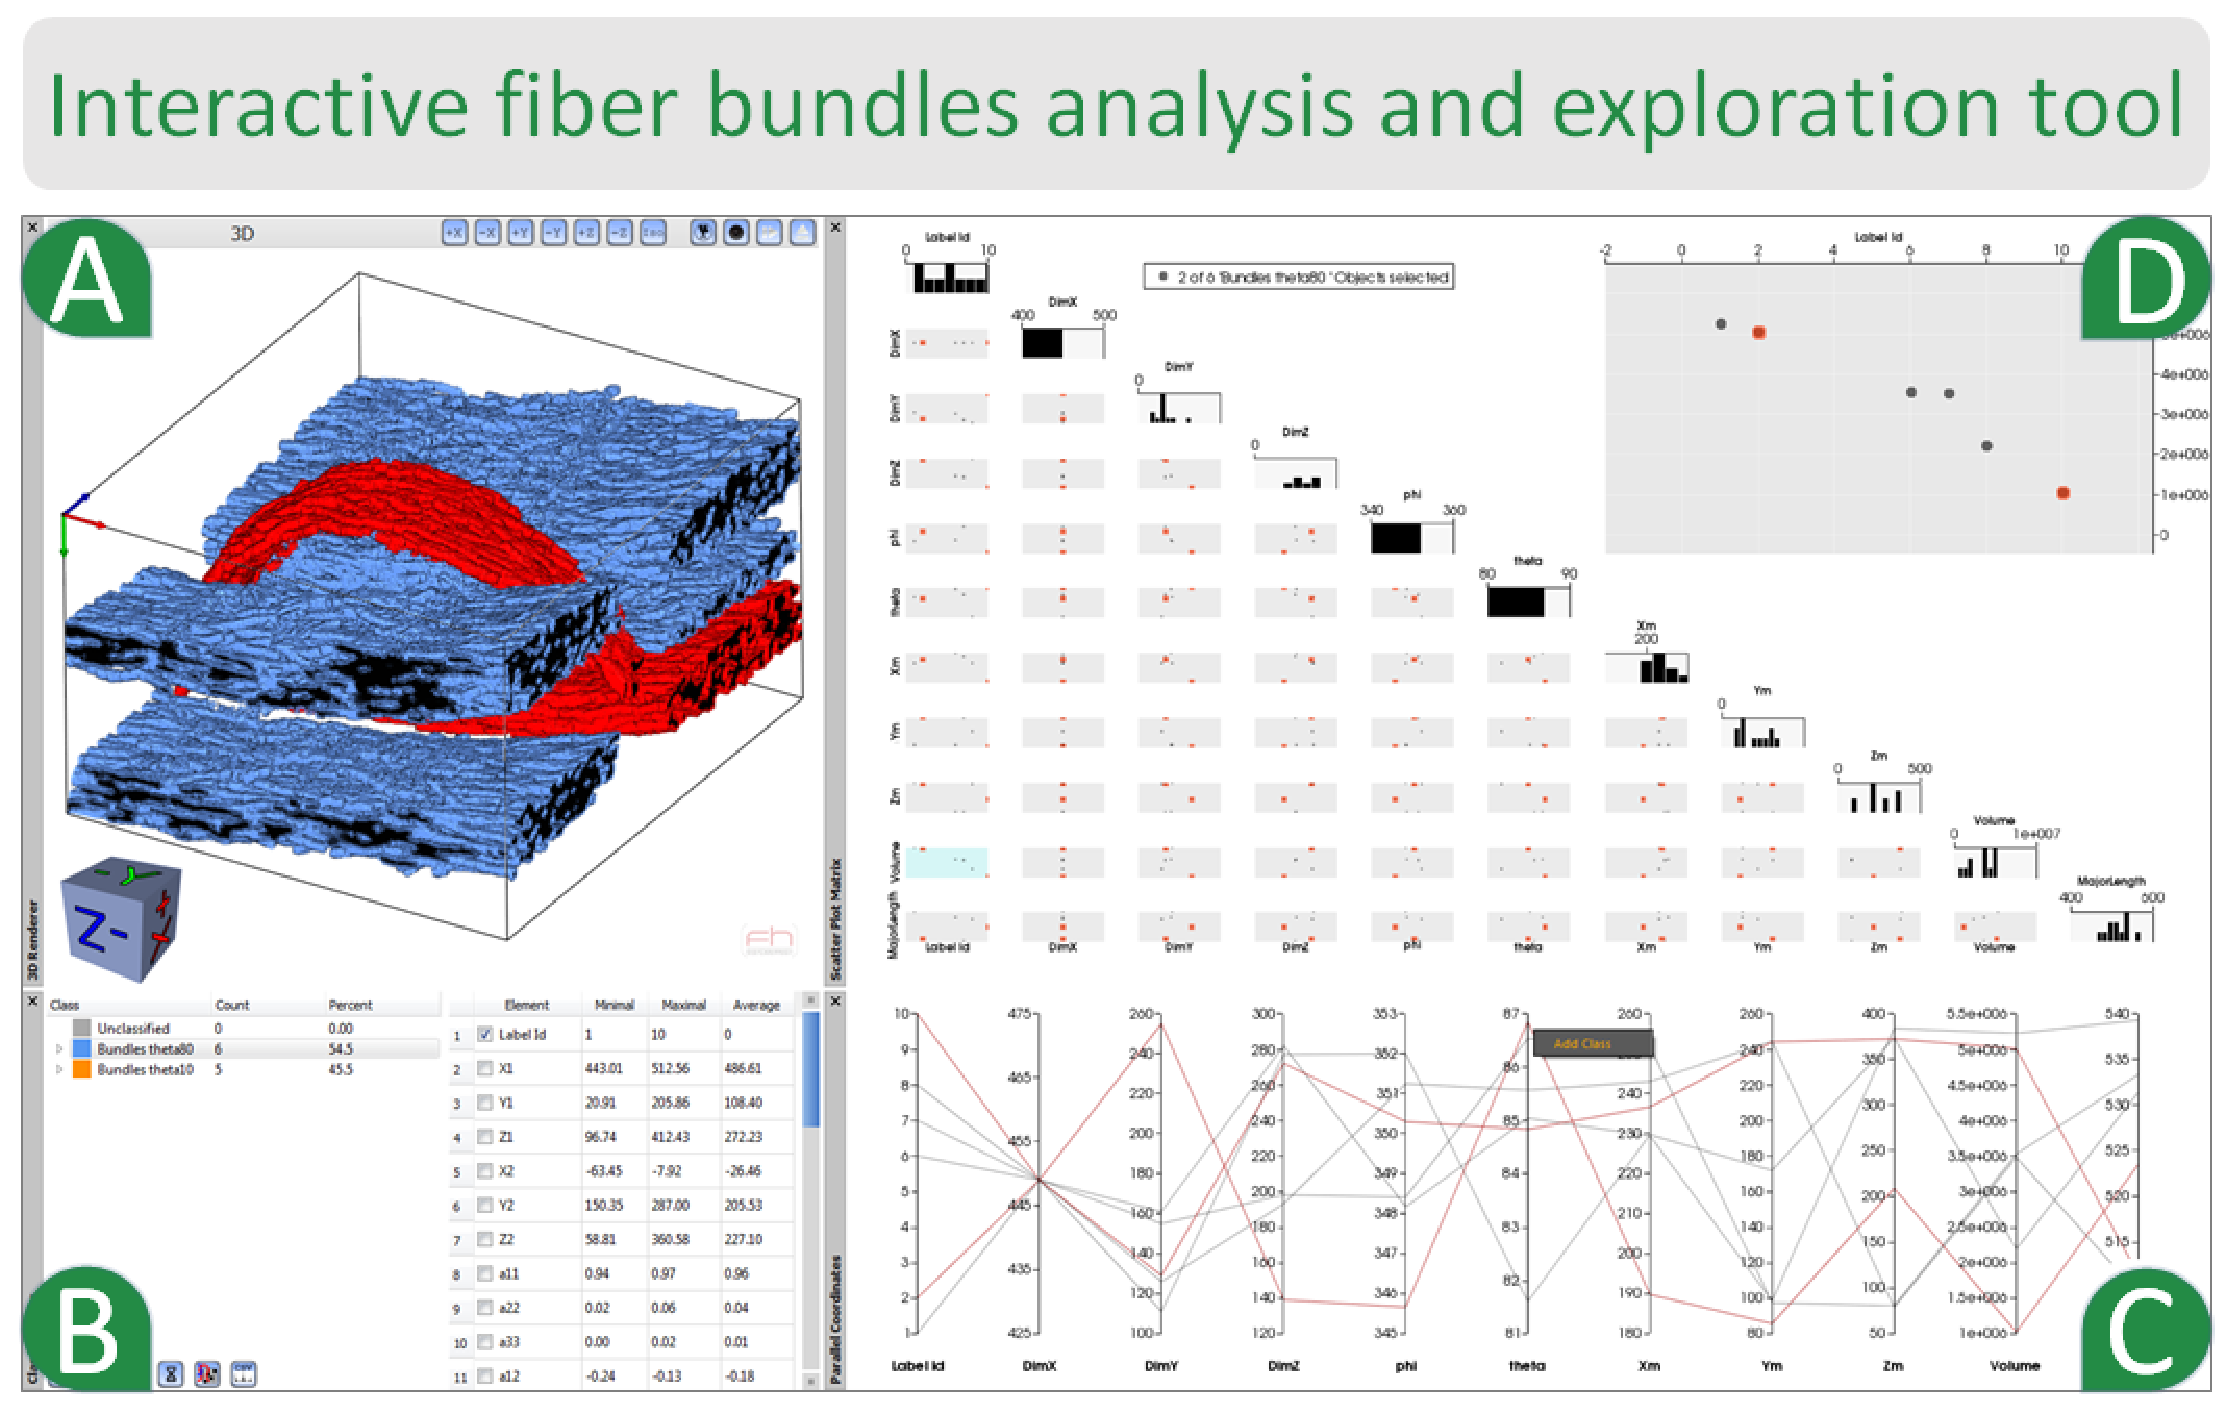
\includegraphics[width=\linewidth]{images/FiberScout_GUI.eps}
	\caption{The interactive graphical user interface for a detailed analysis of fiber bundles generated with a MetaTracts approach. (A) 3D renderer. (B) MetaTracts browser. (C) Parallel coordinates. (D) Scatter plot matrix. \todo{TODO: add more info}}
	\label{fig:interactive_tool_gui}
\end{figure}

\section{User evaluation}\label{sec:user_eval}
\begin{figure}[tb]
	\centering
	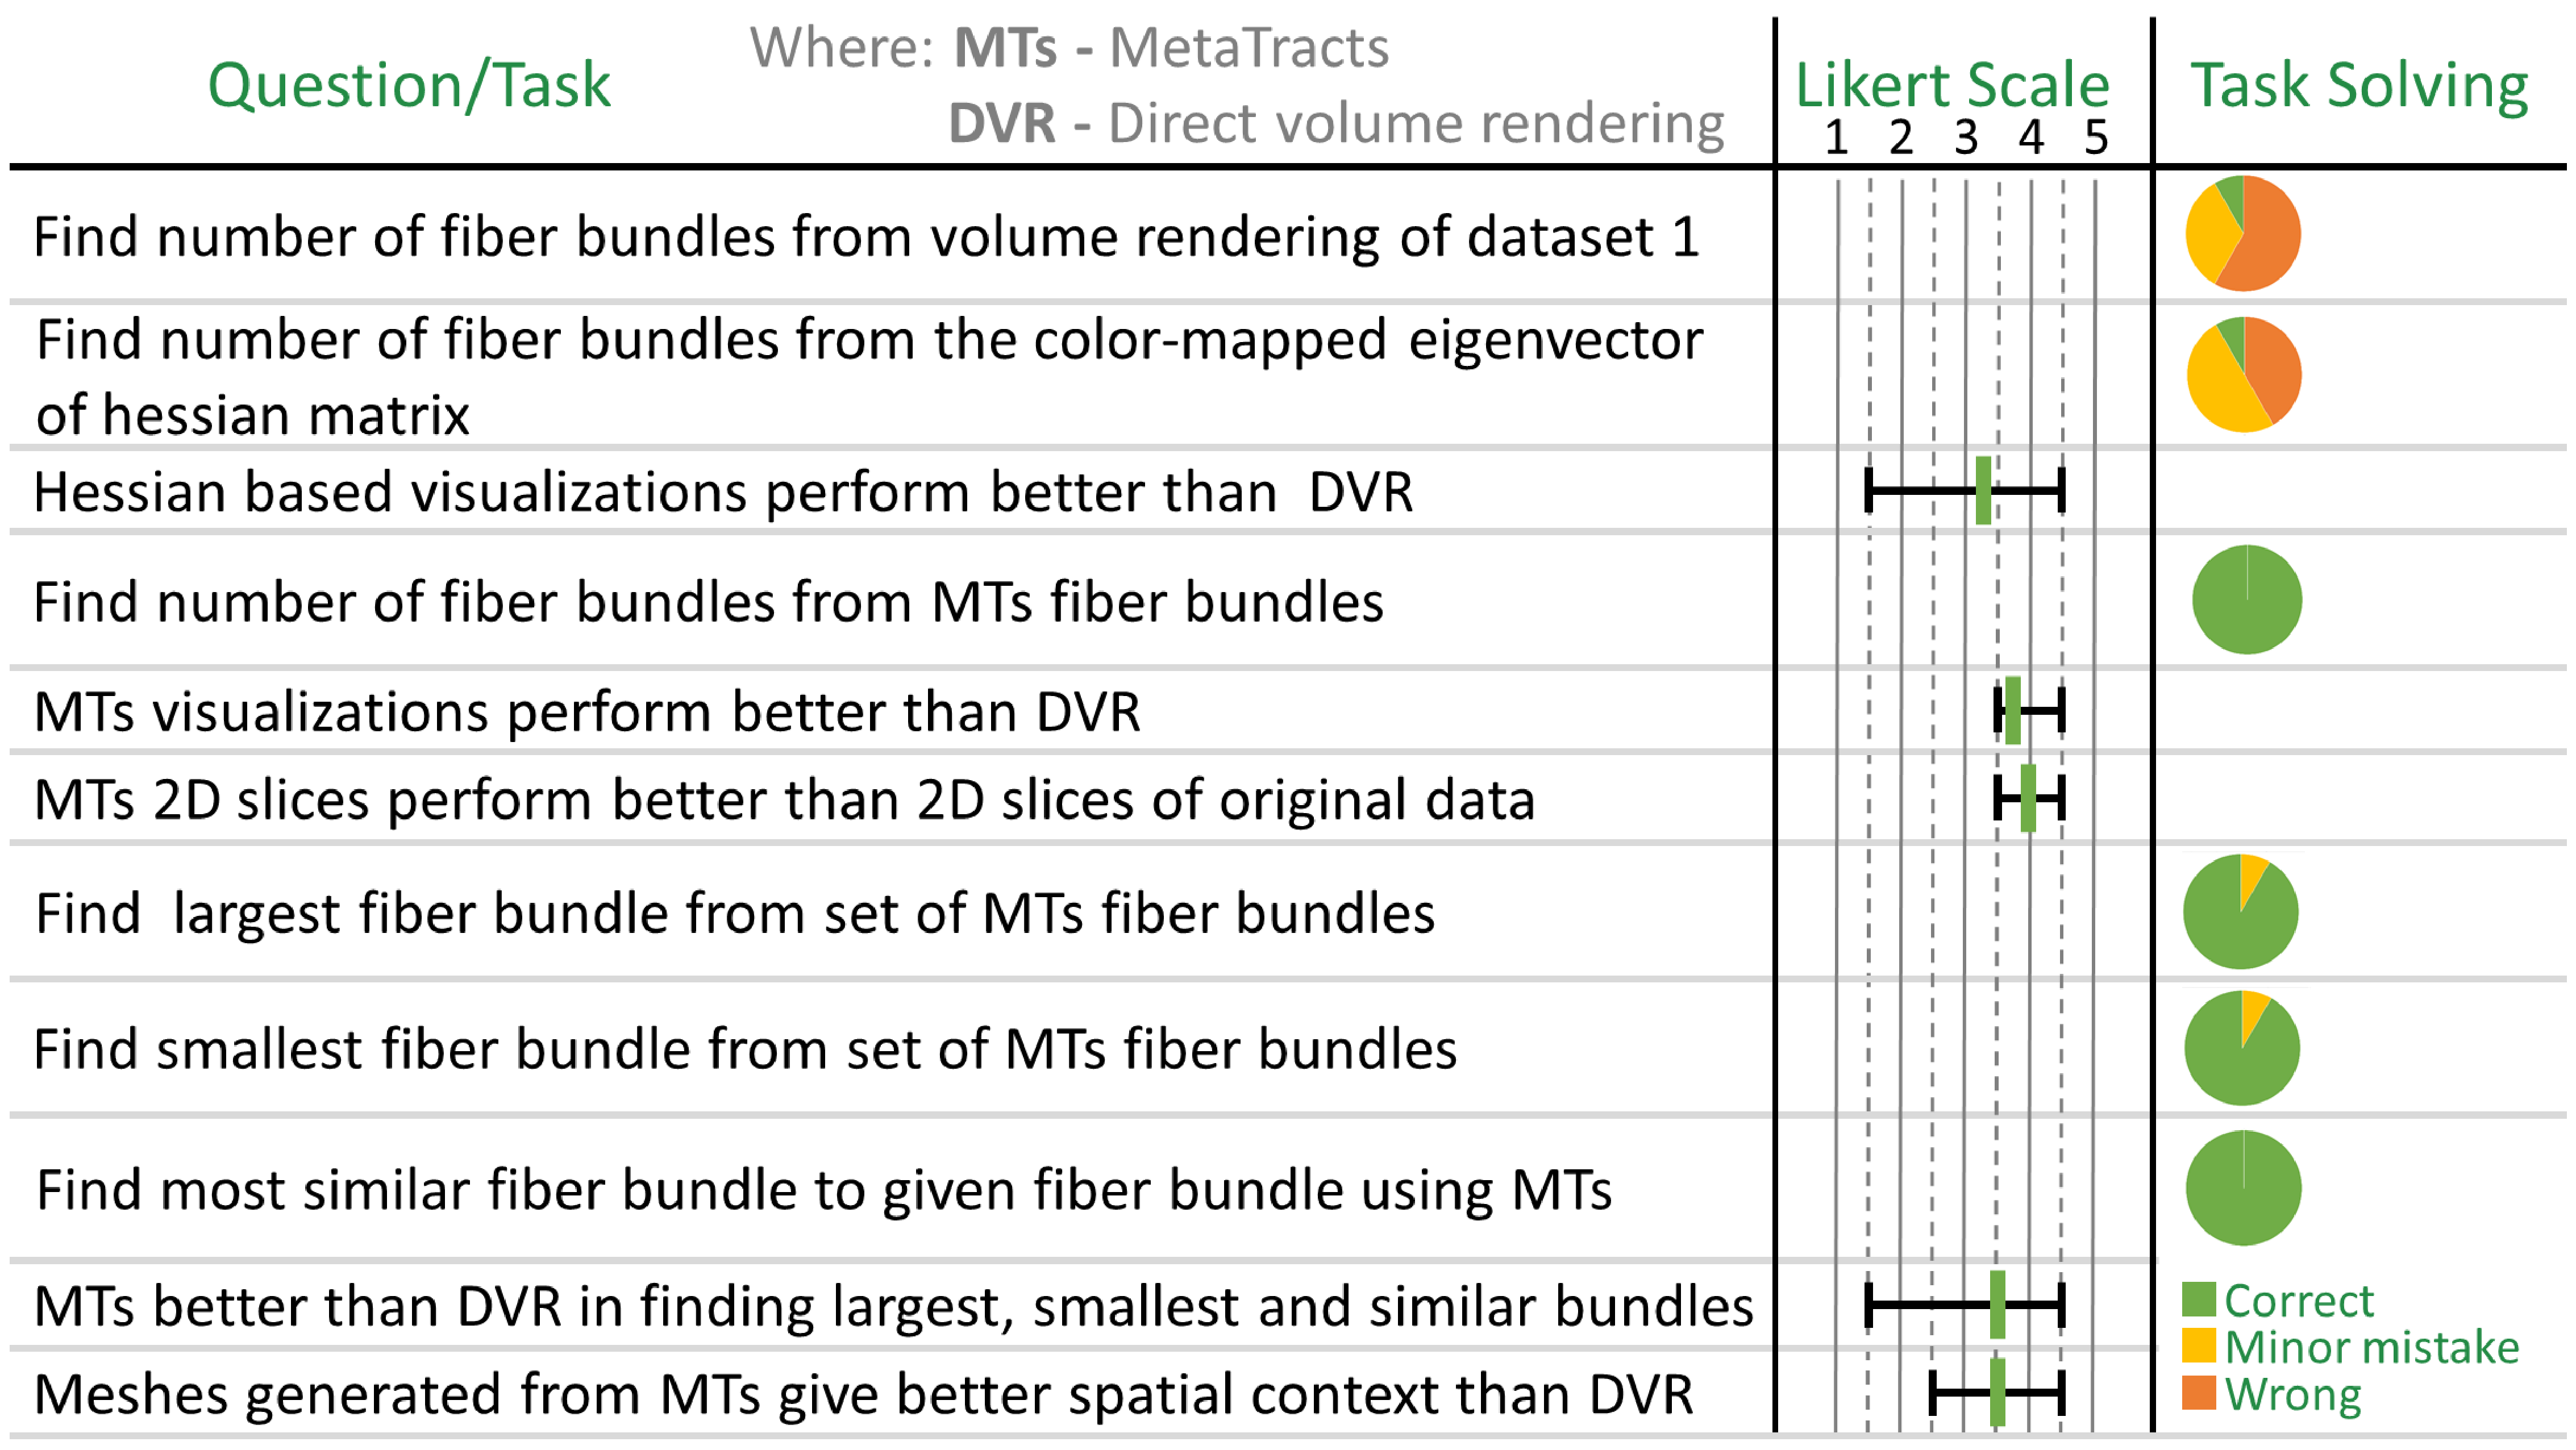
\includegraphics[width=\linewidth,  trim = 0mm 00mm 0mm 0mm, clip]{images/usereval_AMA.eps}
	\caption{The user evaluation consists of a set of queries on videos of our results, volume rendering and Hessian color map. The questionnaire tests the effectiveness of MetaTracts in visualizing ``geometric structure" and ``spatial context". The Likert scale goes from 1-5: strongly disagree, disagree, neutral, agree and strongly agree. }
	\label{fig:userstudy}
\end{figure}
We conducted a user evaluation to test the utility of our technique. Four NDT practitioner working with XCT, four material scientists experienced in analyzing CFRP's and four visualization practitioners participated in the user evaluation of MetaTracts. We set up a questionnaire, with questions on solving given tasks. The queries used Likert Scale (LS) for evaluating the performance of \mt over currently utilized techniques. 
LS consists of 5 levels which range from "strongly agree" to "strongly disagree". Figure~\ref{fig:userstudy} shows the results. The results are presented in the same sequential order that they appeared to the participant. The first set of tasks dealt with the effectiveness of \mt in comprehending ``geometric structure".

 
First we showed the participant a video of full 360{$^\circ$} rotation of the volume rendering of D1 along the Z-axis. We tasked the user to identify the number of separate fiber bundles. The results show that the participants found it difficult to determine the number of fiber bundles from the volume rendering itself. For the second task we mapped the ``top" eigenvector of the Hessian matrix to the RGB color map. We again showed a video of full 360{$^\circ$} rotation of the color-mapped and asked the same query. The Hessian based mapping a popularly used technique in fiber bundle visualization and provides more information about the major orientations than the  gray scale original volume. The results show that the evaluators performed better than the simple volume rendering test (task 1). Majority of our participants agreed or strongly agreed that the Hessian color map was more effective. Finally, we showed the video of the fiber bundles extracted with MetaTracts. 
All participants could correctly identify the number of fiber bundles and agreed that the \mt  is an effective tool for perceiving geometric structure  of fiber bundles, than simple volume rending or Hessian color map. They especially liked the 2D slices of the MetaTracts (Figure~\ref{fig:crop-16-decomp}b, compared to Figure~\ref{fig:data-char}c).

The second set of tasks dealt with the effectiveness of \mt in comprehending ``spatial context".
The participants where given a series of tasks to select fiber bundles which was largest, smallest or most similar to a given fiber bundle from a subset of fiber bundles. In the Likert scale, the majority of the participants agreed that the tasks where easier using \mt than the volume rendering of the original data or using the Hessian color map. 
The majority of the participants also agreed that the extracted meshes provided better spatial context than the volume rendering of the original data. 
